%%%%%%%%%%%%%%%%%%%%%%%%%%%%%%%%%%%%%%%%%
% fphw Assignment
% LaTeX Template
% Version 1.0 (27/04/2019)
%
% This template originates from:
% https://www.LaTeXTemplates.com
%
% Authors:
% Class by Felipe Portales-Oliva (f.portales.oliva@gmail.com) with template 
% content and modifications by Vel (vel@LaTeXTemplates.com)
%
% Template (this file) License:
% CC BY-NC-SA 3.0 (http://creativecommons.org/licenses/by-nc-sa/3.0/)
%
%%%%%%%%%%%%%%%%%%%%%%%%%%%%%%%%%%%%%%%%%

%----------------------------------------------------------------------------------------
%	PACKAGES AND OTHER DOCUMENT CONFIGURATIONS
%----------------------------------------------------------------------------------------

\documentclass[
  french,
  % twocolumn,
	11pt, % Default font size, values between 10pt-12pt are allowed
	%letterpaper, % Uncomment for US letter paper size
	%spanish, % Uncomment for Spanish
]{fphw}

% \usepackage[fontsize=10.0]{scrextend} % Use this to force the fontsize

%% Commands for numbering paragraphs
\renewcommand\thesection{\Roman{section}}
\renewcommand\thesubsection{\thesection.\arabic{subsection}}
\renewcommand*\thesubsubsection{%
  \Roman{section}.\arabic{subsection}.\alph{subsubsection}%
}

\usepackage{sectsty}
\sectionfont{\sf\bfseries\LARGE\raggedright}

% Template-specific packages
% \usepackage{babel}


% \renewcommand*\familydefault{\sfdefault}
\usepackage[utf8]{inputenc} % Required for inputting international characters
% \usepackage{DejaVuSerifCondensed} 
\usepackage[T1]{fontenc} % Output font encoding for international characters
\usepackage{textcomp}

\usepackage[lf]{venturis}
% \usepackage[libertine]{newtxmath}
\usepackage{libertinust1math}
\usepackage{bm} 

\usepackage{fancyvrb}
\usepackage{fvextra}
\newcommand\userinput[1]{\textbf{#1}}
\newcommand\arguments[1]{\textit{#1}}

\usepackage{amsmath}
\usepackage{mathtools}
\usepackage{xfrac} 
% \usepackage{amssymb}
% \usepackage{enumitem}	%% % To modify the itemize bullet character 

\usepackage{graphicx} % Required for including images
\usepackage[textfont=it,font=small]{caption}  %% To manage long captions in images
\usepackage{subcaption}
\captionsetup{justification=centering}

\usepackage{float}
\graphicspath{ {../img/} }

\usepackage{booktabs} % Required for better horizontal rules in tables

\usepackage{listings} % Required for insertion of code

\usepackage{array} % Required for spacing in tabular environment

\usepackage{enumerate} % To modify the enumerate environment

\newcommand{\tabhead}[1]{{\bfseries#1}}

\usepackage{xcolor}
\usepackage{listings}
\colorlet{mygray}{black!30}
\colorlet{mygreen}{green!60!blue}
\colorlet{mymauve}{red!60!blue}

\usepackage[linkcolor=blue,colorlinks=true]{hyperref}
% \usepackage[colorlinks=true,urlcolor=blue]{hyperref}
\hypersetup{citecolor=blue}

\usepackage{cleveref}
\usepackage{siunitx}

\usepackage[backend=bibtex,style=alphabetic,maxnames=2,natbib=true]{biblatex} % Use the bibtex backend with the alphabetic citation style (compact APA-like)
% \usepackage[backend=bibtex,style=authoryear,maxnames=2,natbib=true]{biblatex} % Use the bibtex backend with the authoryear citation style (which resembles APA)
\addbibresource{bibliography.bib} % The filename of the bibliography
\usepackage[autostyle=true]{csquotes} % Required to generate language-dependent quotes in the bibliography 
% \renewcommand*{\bibfont}{\tiny} % Pour reduire la taille des references

\usepackage[useregional=numeric]{datetime2}
\usepackage[normalem]{ulem}

% %-------------------------------------------------------------------------------

\newcommand{\myvec}[3]{\begin{pmatrix} #1  \\ #2 \\ #3 \end{pmatrix}}   %% vecteur 3d
\newcommand{\mymat}[9]{\begin{pmatrix} #1 & #2 & #3 \\ #4 & #5 & #6 \\ #7 & #8 &#9 \end{pmatrix}}  %% Matrice 3*3

\renewcommand{\vector}[4]{\begin{pmatrix} #1  \\ #2 \\ #3 \\ #4 \end{pmatrix}}   %% vecteur 4d
% \newcommand{\mymatrix}[16]{\begin{pmatrix} #1 & #2 & #3 & #4 \\ #4 & #6 & #7 & #8 \\ #9 & #10 & #11 & #12 \\ #13 & #14 & #15 & #16 \end{pmatrix}}  %% Matrice 3*3

\newcommand{\hquad}{\hspace{0.5em}} %% Bew command for half quad
\newcommand*\diff{\mathop{}\!\mathrm{d}}
% \setlength\parindent{0pt}	%% To remove all indentations
\newcommand{\bvec}[1]{\bm{\mathrm{#1}}}  %% Use this to make vectors
\newcommand{\bmat}[1]{\bm{\mathsf{#1}}}   %% Use this to make tensors


%----------------------------------------------------------------------------------------
%	ASSIGNMENT INFORMATION
%----------------------------------------------------------------------------------------

\title{\sf\bfseries Compte rendu semaine \#21} % Assignment title
% \title{Difficultés rencontrées} % Assignment title

\author{Roussel Desmond Nzoyem} % Student name 

\date{\DTMdisplaydate{2021}{6}{23}{-1} - \DTMdisplaydate{2021}{6}{29}{-1}} % Due date

\institute{Sorbonne Université \\ Laboratoire Jacques-Louis Lions} % Institute or school name

\class{Stage M2} % Course or class name

\professor{Pr. Stéphane Labbé} % Professor or teacher in charge of the assignment

%----------------------------------------------------------------------------------------

\begin{document}

\maketitle % Output the assignment title, created automatically using the information in the custom commands above

%----------------------------------------------------------------------------------------
%	ASSIGNMENT CONTENT - INTRO
%----------------------------------------------------------------------------------------

Le travail de cette semaine fut divisé en deux volets bien distincts. Premièrement, il fallait terminer l'interface graphique web pour le problème 2D. Après avoir résolu cette tâche, je suis retourné au problème 1D pour étudier la conservation de l'énergie totale.

%----------------------------------------------------------------------------------------
%	ASSIGNMENT CONTENT - SECTION 1
%----------------------------------------------------------------------------------------

\section*{Tâches effectuées}


\begin{enumerate}
  \item Implémentation d'une interface web adaptée au problème de percussion 2D. Une fois de plus inspirée du travail de Dimitri, on peut voir sur le plot interactif des valeurs propres que le problème est stable (voir \cref{fig:myfig}). 
  \begin{figure}[H]
    \centering
    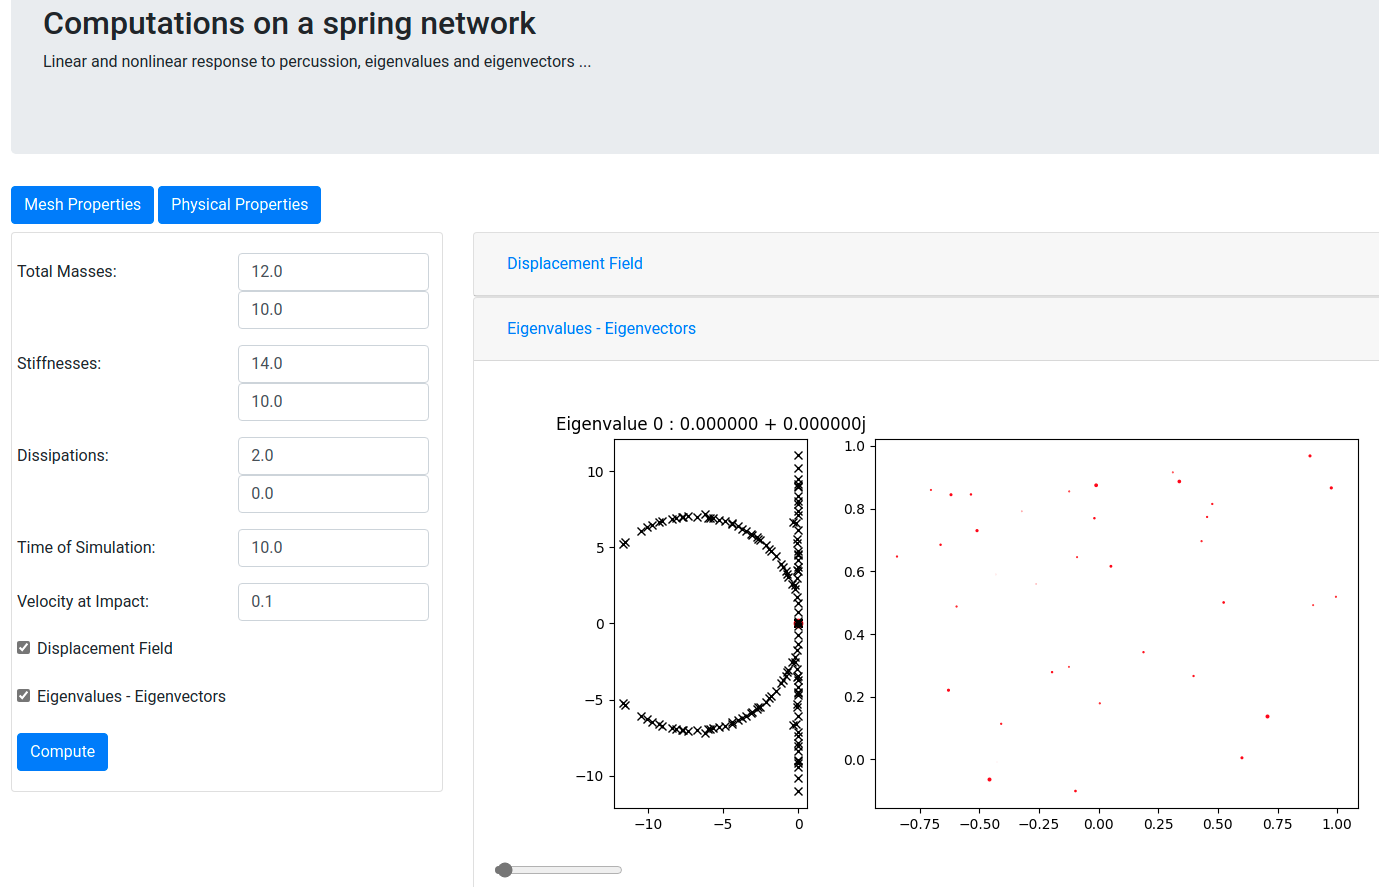
\includegraphics[width=0.60\textwidth]{WebInterface.png}
    \caption{Interface web pour le problème de percusion 2D}
    \label{fig:myfig}
  \end{figure}
  \item La deuxième tâche majeure a été l'étude approfondie de l'énergie totale du système en 1D. Même après avoir décelé une erreur de quadrature dans mes calculs, j'ai du complètement changer le modèle pour avoir la conservation de l'énergie totale. Dorénavant, vu que le système est conservatif (\emph{pour l'instant}), j'applique la conservation de l'énergie cinétique pour déterminer les vitesses après choc (voir \cref{fig:myfig2}, la simulation correspondante est en pièce jointe). 
  \begin{figure}[h]
    \centering
    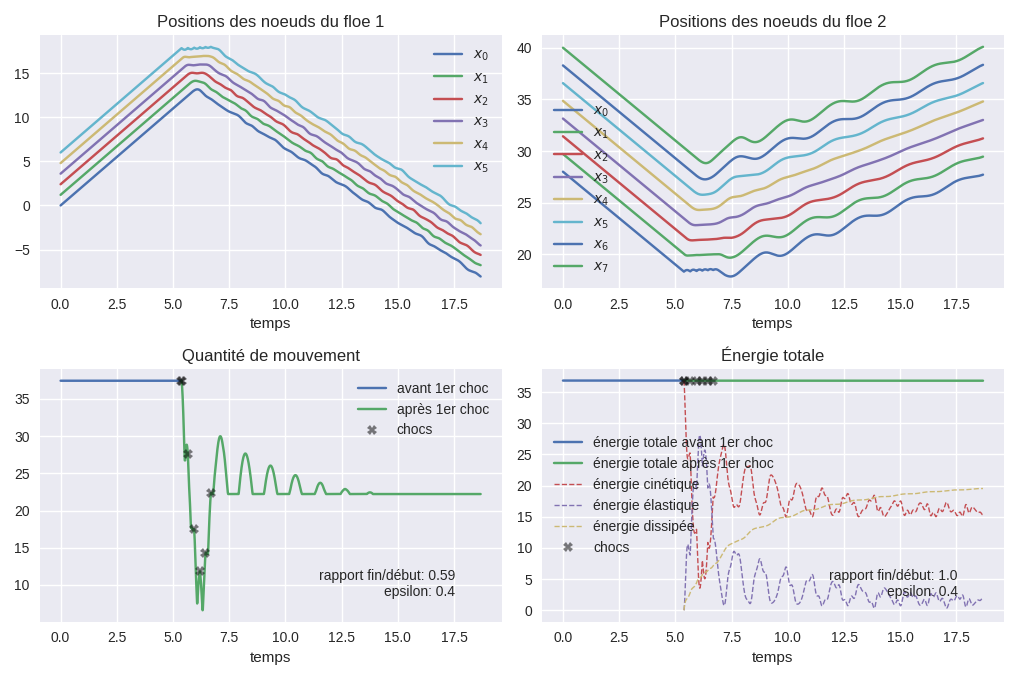
\includegraphics[width=0.60\textwidth]{ImageTot1D.png}
    \caption{Différents graphiques pour la simulation 1D (l'énergie totale est la somme des énergies cinétique, potentielle élastique, et dissipée par frottement visqueux)}
    \label{fig:myfig2}
  \end{figure}
  \item Début d'étude du système 1D à \emph{grande raideur}. Pour l'instant, je ne réussis pas à identifier avec exactitude les noeuds les plus affectés par la percussion (un exemple de simulation à grande raideur est joint à ce rapport).
\end{enumerate}


 
%----------------------------------------------------------------------------------------
%	ASSIGNMENT CONTENT - SECTION 2
%----------------------------------------------------------------------------------------

\section*{Difficultés rencontrées}


\begin{enumerate}
  \item La première est dans l'étude de l'énergie totale du système 1D. J'ai dû changer le modèle en le simplifiant considérablement. En essayant d'écrire le nouveau modèle dans le rapport de stage, je suis indécis : \textbf{dois-je supprimer l'ancien modèle du rapport, ou devrais-je le maintenir pour clairement illustrer mes missions de stage ?} 
  \item La deuxième difficulté est dans l'identification des noeuds les plus affectés par la percussion. Je vois un peu comment aborder le problème au niveau numérique, mais je ne vois pas trop comment le faire au niveau théorique : \textbf{je pensais par exemple regarder le noeuds qui, durant toute la percussion, ont les plus grands déplacements cumulés}, mais je ne suis pas certain.
\end{enumerate}



%----------------------------------------------------------------------------------------
%	ASSIGNMENT CONTENT - SECTION 3
% ----------------------------------------------------------------------------------------
\section*{Travail à venir}

\emph{Par ordre de priorité :}

\begin{enumerate}
  \item Rédaction du nouveau modèle 1D dans le rapport de stage. Concernant le rapport de stage, \textbf{savez-vous s'il y a un délai pour transmettre le document à vous et au laboratoire LJLL pour relecture ?} 
  \item Étude de la condition aux limites 1D.
  \item Étude de la fracturation de la glace dans le modèle 2D.
  \item Étude du schéma symplectique, des valeurs propres du modèle 2D.
\end{enumerate}


 
% %-------------------------------------------------------------------------------
% %							THE BIBLIOGRAPHY
% %-------------------------------------------------------------------------------
\clearpage   % Pour retirer les references de la bare de navigation
% \printbibliography


\end{document}
